\documentclass[12pt]{article}

\usepackage{sbc-template}

\usepackage{graphicx,url}
\usepackage{csvsimple}
\usepackage{subfigure}

\usepackage{multirow}
\usepackage[brazil]{babel}    
\usepackage[utf8]{inputenc}
 
\sloppy

\title{Contagem do número de instruções dos \textit{benchmarks} do
\texttt{SPEC CPU2006} e implementação de novas \textit{pintools}}

\author{Gustavo Ciotto Pinton\inst{1} }


\address{Instituto de Computação -- Universidade Estadual de Campinas
(UNICAMP)\\
  Av. Albert Einstein, 1251, Cidade Universitária, Campinas/SP \\
  Brasil, CEP 13083-852, Fone: [19] 3521-5838
  \email{ra117136@unicamp.br}
}

\begin{document} 

\maketitle

\begin{abstract}
This report describes the number of instructions executed by each
benchmark in \texttt{SPEC CPU2006}. It was achieved thanks to the
Intel's \texttt{pin} application. All results were obtained by running the
benchmarks with the \texttt{ref} inputs and a single iteration. Two new
pin tools were equally developed, capable of listing the number of executed
instructions of every routine of all threads that compose the program and
simulating the 1-bit and 2-bit branch predictor models. Five benchmarks, run
with inputs belonging to the \texttt{ref} set, were used to test these new
tools.
\end{abstract}
     
\begin{resumo} 
Este relatório apresenta o número de instruções executadas por cada
\textit{benchmark} presente no \texttt{SPEC CPU2006}, calculado através da
utilização da ferramenta \texttt{pin}, desenvolvida pela Intel. Os valores
encontrados correspondem às entradas do tipo \texttt{ref} e a uma única
iteração. Além disso, desenvolveu-se duas novas \texttt{pin tools}, cujas saídas
são uma lista com o número de instruções executas pelas rotinas de um
programa, separadas pela sua respectiva \textit{thread}, e o resultado de uma
simulação de dois modelos (\textit{1-bit} e \textit{2-bit}) de \textit{branch
predictor}. Tais ferramentas foram testadas em 5 benchmarks na configuração
\texttt{ref}.
\end{resumo}


\section{Introdução}

\texttt{SPEC}, do inglês \textit{Standard Performance Evaluation Corporation}, é
uma organização constituída por fabricantes de \textit{hardware},
\textit{software} e instuições de pesquisa, cujo objetivo é definir uma série de
testes relevantes e padronizados para a análise da performance de um computador.
Tais testes podem ser igualmente denominados de \textit{benchmarks} e visam
avalisar um aspecto específico de processamento. Durante a aula, vimos que
existe uma grande variedade de \textit{benchmarks} disponíveis na
\textit{internet}, sendo que alguns foram implementados, por exemplo, para
avaliar o desempenho de aplicações \textit{web}. Um \textit{benchmark} realiza
um conjunto de operações definidos, chamado de \textbf{workload}, e produz um
resultado, ou seja, uma \textbf{métrica} que tenta avaliar o desempenho do
computador submetido ao respectivo \textit{workload} \cite{SPEC:11}. Tendo em
vista tais conceitos, o \texttt{SPEC CPU2006} é um conjunto de 31 \textit{benchmarks} que
procuram avaliar a performace de três componentes principais, sendo eles o
processador, a arquitetura de memória e os compiladores. Os \textit{benchmarks}
são distribuídos em dois \textit{suites}, denominados de \texttt{CINT2006} e
\texttt{CFP2006}, que se distinguem quanto à natureza do seu processamento
intensivo: o primeiro é focado na performance das operações que utilizam números
\textbf{inteiros}, sendo que o segundo, de números em \textbf{ponto flutuante}.
Essencialmente, \texttt{SPEC CPU2006} oferece duas métricas, \textbf{speed} e
\textbf{rate} (ou \textbf{throughput}), medindo, respectivamente, o quão rápido
um computador completa uma única tarefa e quantas tarefas tal sistema pode
realizar em um pequeno período de tempo. Cada métrica possui, por sua vez,
quatro \textit{variações}, que se diferenciam quanto ao \textit{suite} (inteiro ou
ponto flutuante) e ao método de compilação. Em relação a este último, duas
opções são disponibilizadas: \texttt{base}, que apresenta requisições mais
estritas, isto é, as \textit{flags} de compilação devem ser usadas na mesma
ordem para todos os \textit{benchmarks} de uma dada linguagem e é exigida para
um teste \textit{reportable} (execução que pode ser publicada), e \texttt{peak}, opcional
e com menos exigências.

\texttt{PIN}, por sua vez, é uma ferramenta para instrumentação e análise de
programas, à medida que ela permite a inserção de código dinamicamente ao
executável. Esta ferramenta é capaz de interceptar a execução da primeira
instrução e gerar um novo código a partir dela. Uma \texttt{pintool} pode ser
definida como uma extensão do processo de geração de código realizada pelo
\texttt{pin}, já que é capaz de interagir com este último e comunicar quais
funções, ou \textit{callbacks}, o aplicativo deve inserir ao código. De maneira
geral, uma \texttt{pintool} é composta por dois componentes, chamados de
\textit{instrumentation code} e \textit{analysis code}. O primeiro deve decidir
onde inserir o novo código, isto é, em que locais as rotinas de análise deverão
ser lançadas. É nessa fase, portanto, que características \textbf{estáticas} do
código, tais como, nome de rotinas ou número de instruções que as
compõem, devem ser exploradas. O segundo, por sua vez, é chamado à medida que o
código é executado e, dessa forma, pode afetar significamente a performance de
um executável se o determinado código apresentar complexidade elevada. 

Neste relatório, será abordada, na primeira parte, o uso de uma \texttt{pintool}
para a avaliação do número de instruções executadas por cada um dos
\textit{benchmarks} e, em seguida, a implementação de duas novas ferramentas
capazes de determinar quantas instruções cada rotina de cada \textit{thread}
foram executadas e de simular a performance de um \textit{branch predictor}.

\section{Contagem das instruções} \label{sec:count}


A fim de calcular as instruções de cada \textit{benchmark} , dois
\textit{scripts bash} foram implementados. O primeiro, chamado de
\texttt{run-pintool-all-benchmarks.sh} verifica e executa o \textit{runspec},
escrito em \textit{perl}, para cada um dos \textit{benchmarks}, além de compilar
a \textit{pintool} que será utilizada. Tal \textit{script} comunica alguns
parâmetros importantes ao comando \textit{runspec}, tais como o método de
compilação (\texttt{base}), o conjunto de entradas que será transmitido aos
programas (\texttt{ref}, no nossa caso), o número de iterações (1) e,
evidentemente, o nome do \textit{benchmark}. A execução deste comando produz um
arquivo de extensão \texttt{.tmp.log} no diretório do projeto, que é copiado
posteriormente a uma pasta, cujo nome é igual ao do \textit{benchmark} que
acabou de ser executado. O arquivo de configuração transmitido ao comando
\texttt{runspec} faz referência ao segundo \textit{script},
\texttt{run-spec-command.sh}, responsável por relacionar o aplicativo
\texttt{pin} com o respectivo \textit{benchmark}. Este \textit{script} recebe
como parâmetro o comando que o \texttt{SPEC} utiliza e o retransmite para o
\texttt{pin}, que é responsável por executá-lo efetivamente.

No manual de referência do \texttt{pin}  \cite{Intel:12}, são indicadas quatro
maneiras distintas de se calcular o número de instruções executadas por um programa. A primeira,
\texttt{inscount0}, insere a rotina de análise antes de cada instrução,
produzindo, assim, uma grande perda de performance. A segunda,
\texttt{inscount1}, é superior à anterior, à medida que utiliza uma outra medida
de granularidade, chamado de \texttt{BBL} (do inglês, \textit{basic block}) e,
portanto, economiza diversas chamadas à função de análise. A terceira rotina,
chamada de \texttt{inscount2}, usa o mesmo princípio que a anterior, porém
apresenta melhor desempenho, visto que faz uso de dois recursos a mais que
\texttt{inscount1}. O primeiro recurso é a mudança de \texttt{IPOINT\_BEFORE}
para \texttt{IPOINT\_ANYWHERE}, que autoriza o \texttt{pin} escolher em que
ordem a função de análise é colocada, permitindo, assim, que ele escolha o ponto
que requeira mínimas operações de salvamento e restaturação dos registradores.
Além disso, esta ferramenta também usa a opção de \textit{fast call linkage},
que explora o fato de que alguns compiladores podem eliminar o
\textit{overhead} que, para funções pequenas como a a função de análise, é
comparável ao próprio conjunto de operações da respectiva função. Esta opção é
ativada através do uso de \texttt{PIN\_FAST\_ANALYSIS\_CALL}. Por fim, o último
programa utiliza, além dos recursos comentados anteriormente, uma unidade de
armazenamento rápido, chamado de \texttt{TLS}, indexado pelos \textit{indexes}
das \textit{threads} para gerar o número de instruções por \textit{thread}. 

Tendo em mente estas características, escolhe-se o programa
\textbf{\texttt{inscount2}} para o cálculo do número de instruções, visto que
este último apresenta o maior número de otimizações e que, neste contexto, não
visa-se encontrar uma contagem por \textit{threads}, mas sim global. Os
\textit{benchmarks} foram rodados em apenas um \textit{core} do processador
\textit{Intel i3} e levaram, ao todo, 20 horas aproximadamente. Os resultados
encontrados estão listados abaixo. Alguns \textit{benchmarks} possuem mais de
uma entrada e, portanto, produzem mais de uma saída. Tais saídas estão
representadas por barras de cores distintas nas figuras a seguir, sendo que a
primeira execução corresponde à barra mais próxima da extremidade esquerda e a
última, à mais próxima do canto direito.
A figura 1 representa a contagem para os \textit{benchmarks} presentes no
conjunto \texttt{CINT2006}, enquanto que os da figura \ref{fig:cfp} ao \texttt{CFP2006}.

% Para os \textit{benchmarks} do conjunto \textbf{inteiro}:
% \begin {itemize}
% \item \texttt{400.perlbench}: 1109199453135, 384794966180 e 707786630078;
% \item \texttt{401.bzip2}: 432459815466, 181180973754, 309587458388,
% 553737482083, 605707320979 e 345617094417;
% \item \texttt{403.gcc}: 77486081001, 151304896042, 139516901551, 103544794782,
% 113969110763, 154632720603, 183464085374, 169988864190 e 58464730027;
% \item \texttt{429.mcf}: 341546845898;
% \item \texttt{445.gobmk}: 234525646891, 625630912777, 325147400011, 235593270689
% e 339210184746;
% \item \texttt{456.hmmer}: 971544936415 e 2052353062716;
% \item \texttt{458.sjeng}: 2309967981602;
% \item \texttt{462.libquantum}: 2291912513237;
% \item \texttt{464.h264ref}: 500835844419, 355915755256 e 3188039031373;
% \item \texttt{471.omnetpp}: 576120751009;
% \item \texttt{473.astar}: 411719281496 e 829803428219;
% \item \texttt{483.xalancbmk}: 1048497777430;
% \end {itemize}

\begin{figure}[h!]
\centering
  \centering
  \label{fig:cint}
  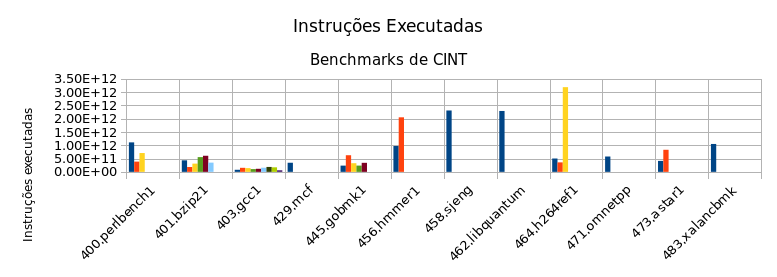
\includegraphics[width=0.9\linewidth]{cint}
  \caption{Número de instruções dos \textit{benchmarks} pertencentes ao conjunto \texttt{CINT}.}
\end{figure}

\vspace{-12pt}

\begin{figure}[h!]
  \centering
  \label{fig:cfp} 
  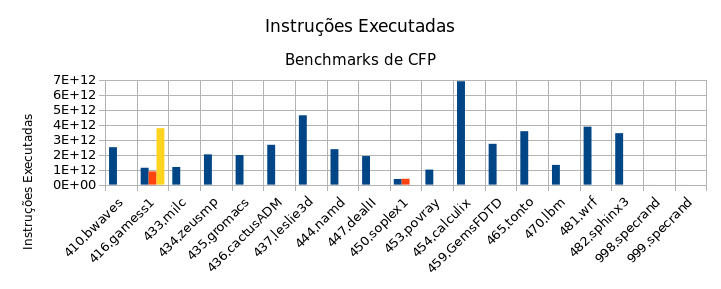
\includegraphics[width=0.9\linewidth]{cfp}
  \caption{Número de instruções dos \textit{benchmarks} pertencentes ao conjunto \texttt{CFP}.}
\end{figure}


%Para os \textit{benchmarks} do conjunto em \textbf{ponto flutuante}:
% \begin {itemize}
% \item \texttt{410.bwaves}: 2495514310671;
% \item \texttt{416.gamess}: 1124505751802, 878108822120 e 3766238102301;
% \item \texttt{433.milc}: 1175358807602;
% \item \texttt{434.zeusmp}: 2016616007500;
% \item \texttt{435.gromacs}: 1971200720105;
% \item \texttt{436.cactusADM}: 2655006820074;
% \item \texttt{437.leslie3d}: 4626149683194;
% \item \texttt{444.namd}: 2361163843397;
% \item \texttt{447.dealII}: 1903231296730;
% \item \texttt{450.soplex}: 377422013533 e 389471401592;
% \item \texttt{453.povray}: 1002527860013;
% \item \texttt{454.calculix}: 6894341859256;
% \item \texttt{459.GemsFDTD}: 2722718843589;
% \item \texttt{465.tonto}: 3563812436773;
% \item \texttt{470.lbm}: 1314569317678;
% \item \texttt{481.wrf}: 3867428096173;
% \item \texttt{482.sphinx3}: 3432419178361;
% \item \texttt{998.specrand}: 536611748;
% \item \texttt{999.specrand}: 536611748;
% \end{itemize}

Verifica-se, portanto, que o \textit{benchmark} que utiliza mais entradas em
seus testes é \texttt{403.gcc}, com 9 entradas, totalizando 1.152.387.847.873
instruções executadas. Os \textit{benchmarks} que rodaram mais e menos instruções foram,
respectivamente, \texttt{454.calculix} (com 6.894.341.859.256 instruções) e
\texttt{998.specrand}/\texttt{999.specrand} (tendo 536.611.748 instruções cada). 


\section{Implementação de novas \textit{pin tools}} \label{sec:tool}

Nesta seção, serão discutidas as duas novas \textit{pin tools} desenvolvidas.

\subsection{Contagem de instruções por \textit{thread} e por rotina}

Tendo em vista que os programas apresentados na seção anterior não permitem a
contagem de instruções por rotina e por \textit{thread}, propõe-se a
implementação de uma nova \textit{pintool} contendo estas duas funcionalidades.
Para isso, utiliza-se a API da ferramenta para a adição de funções de
\textit{instrumentação} para cada rotina e de \textit{análise} para suas
instruções. Além disso, faz-se uso do \textit{TLS} para a armazenagem de
informações específicas a uma \textit{thread}.

O registro da função de instrumentação é realizada através de uma chamada a
\texttt{RTN\_AddInstrumentFunction()}, cujo  parâmetro é uma
\textit{callback function} que é executada uma vez para cada rotina do
programa. Dentro desta função, processa-se todo o comportamento estático do
programa, isto é, explora-se o seu estado independente da sua execução. Cada
rotina é descrita por uma estrutura de dados, cujo nome é \texttt{RTN}. Tal
estrutura permite que diversas informações sejam extraídas, como por exemplo, o
nome da rotina, através de \texttt{RTN\_Name()}, o número de instruções
estáticas dentro dela, com \texttt{RTN\_NumIns()} e quais instruções pertencem a
ela. Este último é realizado através da iteração de uma lista ligada, acessada
através de \texttt{RTN\_InsHead()} ou \texttt{RTN\_InsTail()}. No entanto, tais
funções devem ser chamadas somente depois de \texttt{RTN\_Open()} ser executada,
conforme documentado no manual da ferramenta  \cite{Intel:12}.

O programa define duas novas classes, \texttt{Thread\_node} e
\texttt{Routine\_node}, responsáveis por armazenar informações sobre as
\textit{threads} e rotinas executadas. Os objetos instanciados destas classes
compõem duas listas ligadas, sendo que cada nó do tipo \texttt{Routine\_node}
contém o início e o fim de uma lista de objetos \texttt{Thread\_node}. Tal
escolha de implementar uma lista de \texttt{Thread\_node} dentro de cada
instância de \texttt{Routine\_node}, e não o inverso, foi adotada a fim de
melhorar a performance da rotina de análise, que será explicada mais adiante.
Além de dois ponteiros para o início e fim de uma lista ligada de
\texttt{Thread\_node}s, um objeto da classe \texttt{Routine\_node} possui o nome
da rotina, obtido através de \texttt{RTN\_Name()}, a referência para o próximo
nó da lista e o \textit{id}, que é dado pela função \texttt{RTN\_Id()}.
\texttt{Pin} atribui a cada rotina uma identificação única globalmente, isto é, 
mesmo se uma determinada rotina com mesmo nome aparecer em duas imagens distintas,
as duas \textit{cópias} terão \textit{ids} diferentes. Um objeto da classe
\texttt{Thread\_node} possui, por sua vez, além de um ponteiro para o próximo
elemento da lista, o \textit{id} da \textit{thread}, que pode ser recuperado
através do \texttt{THREAD\_ID} e o número de instruções que a rotina daquela
respectiva \textit{thread} executou.

A criação de nós do tipo \texttt{Routine\_node} é realizada na rotina de
instrumentação por motivos ligados à performance, visto que é um processo
extremamente custoso. Tal afirmação reside no fato de que uma rotina
pode aparecer mais de uma vez em \textit{threads} distintas e que, por este
motivo, é necessário percorrer a lista toda vez a fim de procurá-la. Observa-se
também que um programa pode apresentar um número elevado de rotinas - os
\textit{benchmarks} testados, por exemplo, apresentam mais de 1000 delas. Dessa
forma, caso tais operações fossem inseridas na função de análise, a performance
do programa seria afetada muito negativamente. Sendo assim, após a verificação
da existência da rotina na lista e a possível criação em caso negativo,
inicia-se o processo de posicionamento das funções de análise. Cada estrutura do
tipo \texttt{RTN} possui uma referência para uma lista das instruções que a
compõem, sendo acessada pela função \texttt{RTN\_InsHead()} e percorrida por
\texttt{RTN\_Next()}. Para cada instrução, executa-se, portanto, a função
\texttt{INS\_InsertCall()} para inserir a \textit{callback} de análise. Essa
função pode receber, além da referência da \textit{callback}, a ordem em que
ela é chamada (antes ou depois, por exemplo, da execução da instrução) e um
conjunto variável de parâmetros. \texttt{PIN} oferece uma série de
possibilidades para a passagem de parâmetros à função de análise. No nosso caso,
por exemplo, dois argumentos são utilizados, sendo eles o \textit{id} da
\textit{thread}, que é passado através de \texttt{THREAD\_ID}, definido na
enumeração \texttt{IARG\_TYPE}, e o ponteiro do objeto do tipo
\texttt{Routine\_node}, que identifica a qual rotina a instrução pertence. Este
último exige a adição de dois parâmetros a \texttt{INS\_InsertCall()}: um para a
especificação do tipo do argumento, isto é, \texttt{IARG\_PTR}, e o segundo o
ponteiro propriamente dito. Para a ordem de execução, quatro opções são
disponíveis, sendo elas \texttt{IPOINT\_BEFORE}, \texttt{IPOINT\_AFTER} ,
\texttt{IPOINT\_ANYWHERE} e \texttt{IPOINT\_TAKEN\_BRANCH}, equivalendo,
respectivamente, à execução da rotina de análise antes, depois, em um ponto
determinado pelo próprio \texttt{PIN} ou se um \textit{branch} foi executado.
Como não há nenhuma preferência de ordem e prefere-se aquela que ofereça melhor
desempenho, escolhe-se \texttt{IPOINT\_ANYWHERE}.

Por último, a criação de nós do tipo \texttt{Thread\_node} é realizada na função
de análise juntamente com o incremento do número de instruções executadas. É 
necessário, porém, a fim de não comprometer siginificamente a execução do
programa, implementarmos uma função que execute o mínimo de operações. Neste
contexto, acessa-se a lista de \texttt{Thread\_node}s através do ponteiro do
tipo \texttt{Routine\_node}, passado como parâmetro, e procura-se o nó, cujo
\textit{id} seja igual ao segundo argumento da função. Caso ele não seja
encontrado, um novo nó é criado. Vale lembrar, portanto, que o desempenho do
programa é fortemente prejudicado caso ele possua muitas \textit{threads}. Isso
porque a lista ligada de \texttt{Thread\_node}s é sempre percorrida a cada nova
instrução. Por fim, o contador de instruções é incrementado.

Esta \texttt{pintool} foi testada em cinco \textit{benchmarks} do
\texttt{SPEC CPU2006}, sendo eles \texttt{400.perlbench}, \texttt{401.bzip2},
\texttt{403.gcc}, \texttt{429.mcf}  e \texttt{445.gobmk}. A impressão dos resultados é
realizada de maneira decrescente. A seguir, são apresentadas algumas
considerações importantes a respeito das execuções.

\begin {itemize}
  \item Todos os \textit{benchmarks} \textbf{testados} apresentam apenas uma
  \textit{thread}, portanto a sua performance não é \textit{extremamente}
  degradada pela \textit{tool};
  \item A execução de \texttt{malloc} corresponde a apenas 0.34\% das instruções
  executadas por \texttt{400.perlbench};
  \item A routina que é mais executada em \texttt{401.bzip2} é
  \texttt{BZ2\_compressBlock}, sendo executada 0.7\% das vezes;
  \item as instruções executadas em \texttt{htab\_traverse} valem 1.77\% do
  número de instruções de \texttt{403.gcc};
  \item \texttt{update\_tree} corresponde a 1.09\% da execução de
  \texttt{429.mcf};
  \item \texttt{445.gobmk} chama, em média, 1664 rotinas.  
\end{itemize}

\subsection{Simulação dos modelos de 1 e 2 \textit{bits} de \textit{branch
predictor}}

A segunda ferramenta implementada utilizou os recursos do \texttt{pin} para
avaliar a performance de dois \textit{branch predictors}, sendo eles de 1 e dois
\textit{bits}. Para isso, três novas classes foram implementadas. A primeira,
\texttt{GenericBP}, é abstrata e serve como modelo para as demais classes, que
devem implementar o método \texttt{update}, que recebe como parâmetro um
endereço de 32 \textit{bits} e recalcula os estados do preditor. A segunda
classe, \texttt{BP1bit}, implementa um preditor de um \textit{1 bit}, isto é,
que utiliza apenas o resultado do último evento para a sua atualização. Por fim,
a classe \texttt{BP2bit} define o modelo de \textit{2 bits} que utiliza uma
máquina com 4 estados possíveis. A instrumentação é realizada a cada instrução
de pulo ou chamada de função, sendo implementada através das funções
\texttt{INS\_IsDirectBranchOrCall}, capaz de retornar se uma instrução atende a
essa condição, e \texttt{INS\_InsertCall}, já discutida anteriormente. Três
parâmetros são passados à função de análise, sendo eles o endereço PC da
instrução de pulo ou chamada, seu endereço alvo e se o pulo foi realizado. Tais
parâmetros são especificados através de, respectivamente,
\texttt{INS\_Address}, \texttt{INS\_DirectBranchOrCallTargetAddress} e
\texttt{IARG\_BRANCH\_TAKEN} durante a chamada de \texttt{INS\_InsertCall}.

A execução desta \textit{pintool} nos mesmos \textit{benchmarks} da subseção
anterior permitiu a avaliação dos dois modelos. Como esperado,
o modelo de 2 \textit{bits} sempre superou o de 1 \textit{bit}. A tabela
\ref{tab:modelos} mostra os resultados para os dois modelos de \textit{branch
predictor}. \textit{Entrada} corresponde ao número de entradas de cada
\textit{benchmark}, \textit{Misses} é a somatória do número de
\textit{miss-predictions} de todas as entradas, \textit{Hits} a somatória das
quantidades em que o preditor acertou e, enfim, \% é a razão 
\(\frac{Hits}{Hits+Misses}\). Tais campos são as médias dos resultados de todas
as entradas.

 \begin{table}[h]
    \centering
	\caption{\label{tab:modelos} Resultados obtidos para os modelos \textit{1-bit}
	e \textit{2-bit}.}
	\begin{tabular}{ c | c | c | c | c | c | c | c |}
		\hline
		\multicolumn{2}{c|}{} & \multicolumn{3}{c|}{\textbf{Modelo 1}} &
		\multicolumn{3}{c|}{\textbf{Modelo 2}}	\\ 	\hline 
		\textit{\textbf{Benchmark}} & Entradas  & \textit{Misses} & \textit{Hits} & \%
		& \textit{Misses} & \textit{Hits} & \% \\
		\hline \hline \texttt{400.perlbench} & 3 & \(4.0\times10^{10}\) &
		\(9.4\times10^{10}\) & 0.70 & \(2.7\times10^{10}\) & \(1.1\times10^{11}\)
		& 0.80
		\\
		\hline \texttt{401.bzip2} & 6 & &  & & & \\ \hline 
		\texttt{403.gcc} & 9 & & & & & \\
		\hline \texttt{429.mcf} & 1 & & & & & \\ \hline 
		\texttt{445.gobmk} & 5 & & & & & \\ \hline 		
	\end{tabular}	    
\end{table} 


\section{Conclusões}

Neste relatório, explorou-se algumas funcionalidades do \texttt{pin}, aliado
com a execução dos \textit{benchmarks} contidos no \texttt{SPEC CPU 2006}. Foi
possível avaliar, portanto, quais \textit{benchmarks} utilizaram mais
ou menos instruções durante sua execução. Além disso, foi possível verificar
que alguns deles rodaram mais de uma vez com entradas diferentes, uma vez que o número de
instruções variou. Adicionalmente, implementou-se duas \textit{pintools} para
extender as funcionalidades dos exemplos dados na página de referência da ferramenta e para
explorar os conceitos de \textit{branch prediction} discutidos em aula.
Estas novas \textit{pintools} exploraram, diversos recursos da API e são
capazes, respectivamente, de imprimir as rotinas de cada \textit{thread} em ordem
decrescente, permitindo, assim, o estudo das rotinas que mais impactam a aplicação
avaliada, e de contar o número de vezes que os modelos de 1 e 2 \textit{bits}
foram bem-sucedidos na predicação na execução dos \textit{benchmarks}.


\bibliographystyle{sbc}
\bibliography{sbc-template}

\end{document}